\begin{figure}[!t]
		\begin{center}
%			\subfloat[]{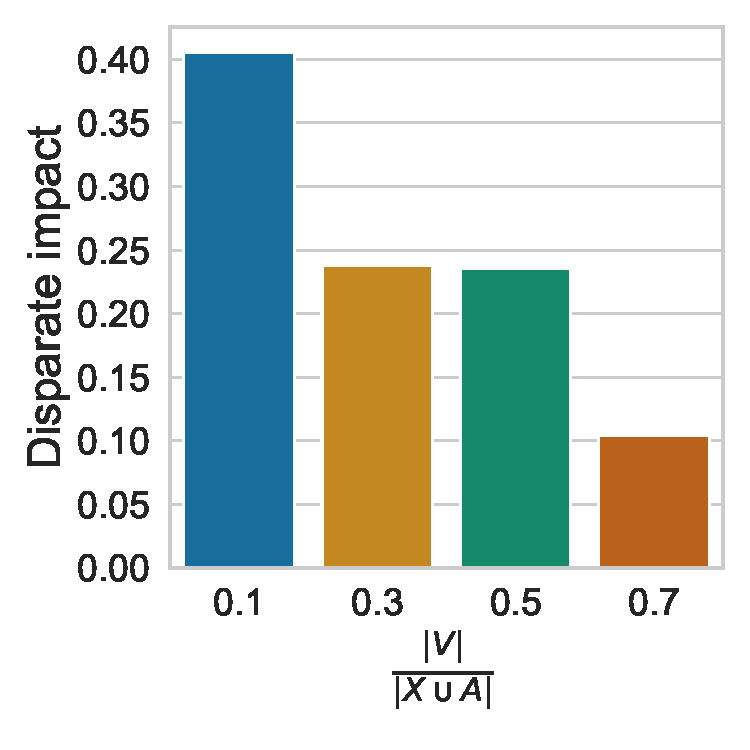
\includegraphics[scale=0.25]{figures/dag_complexity_DAG_DI_Adult_LR_sex__age}}
%			\subfloat[]{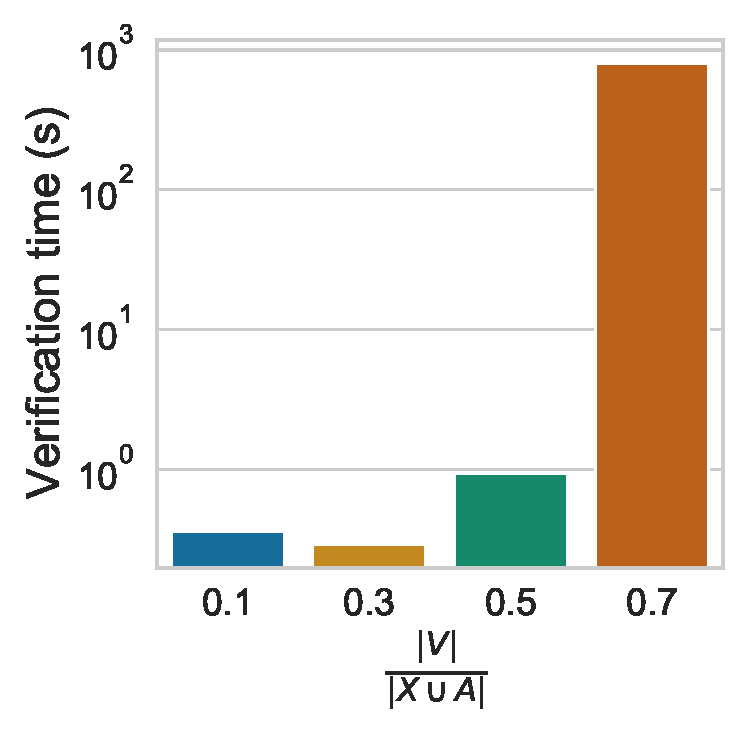
\includegraphics[scale=0.25]{figures/dag_complexity_DAG_time_Adult_LR_sex__age}}
%			\subfloat[]{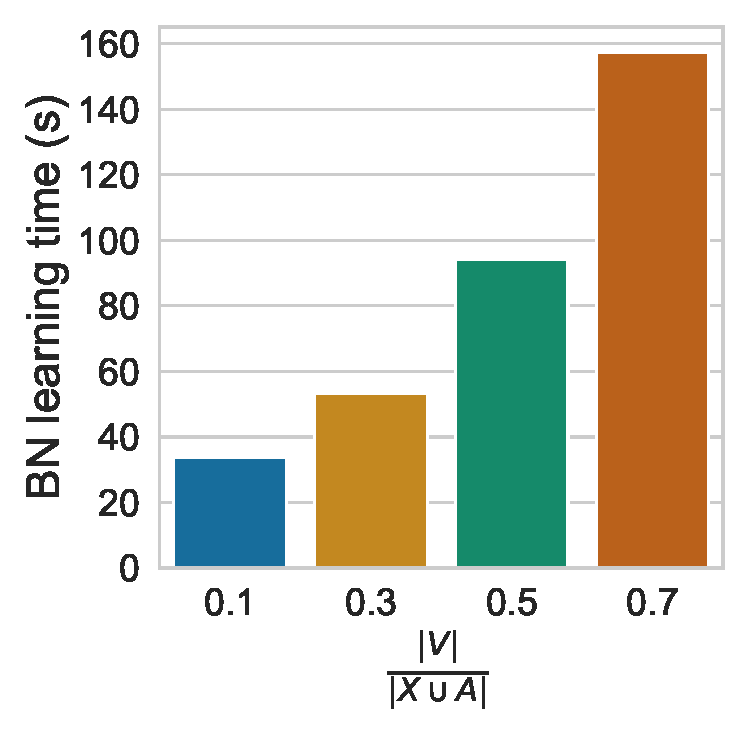
\includegraphics[scale=0.25]{figures/dag_complexity_DAG_time_notears_Adult_LR_sex__age}}
%
%
%			\subfloat[]{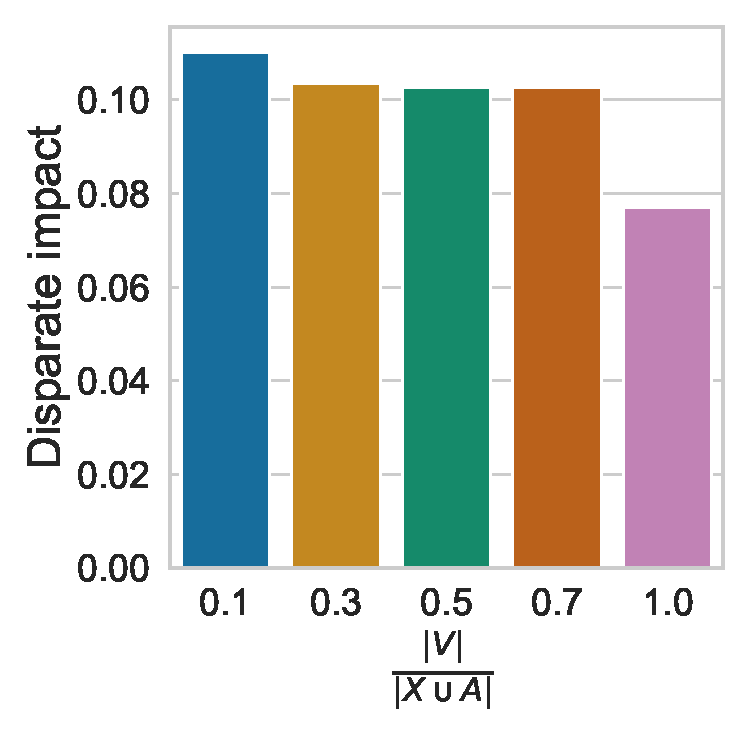
\includegraphics[scale=0.25]{figures/dag_complexity_DAG_DI_Compas_LR_age__sex}}
%			\subfloat[]{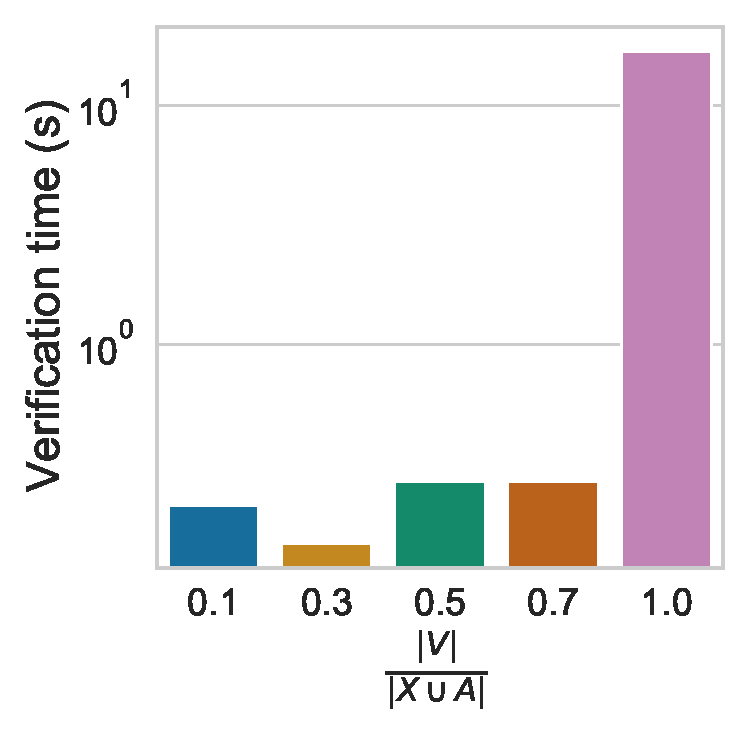
\includegraphics[scale=0.25]{figures/dag_complexity_DAG_time_Compas_LR_age__sex}}
%			\subfloat[]{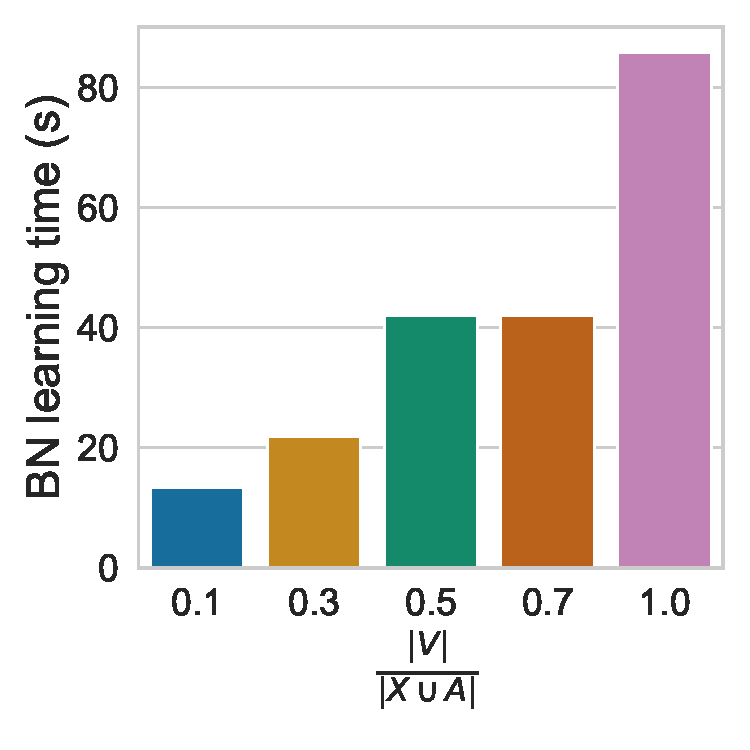
\includegraphics[scale=0.25]{figures/dag_complexity_DAG_time_notears_Compas_LR_age__sex}}
%			
%			
%			\subfloat[]{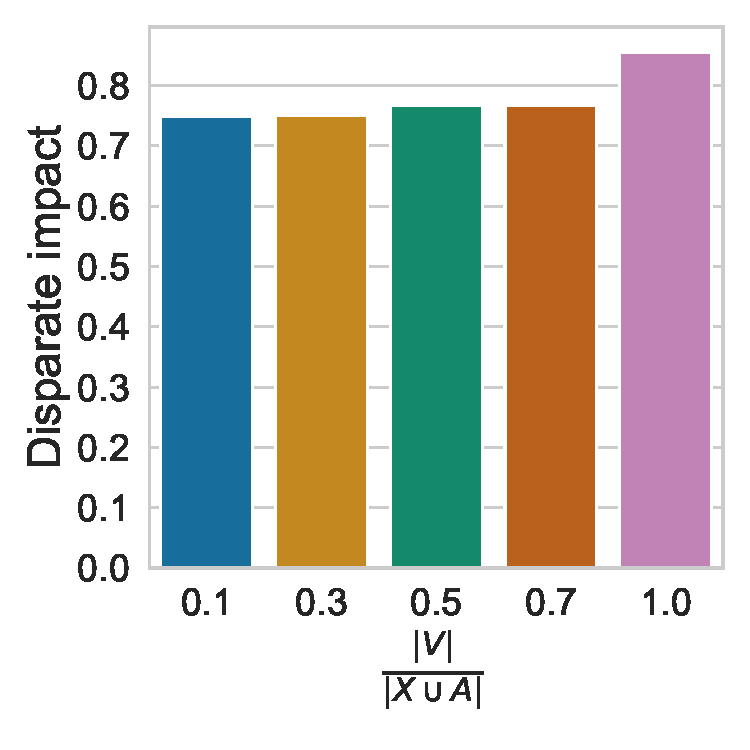
\includegraphics[scale=0.25]{figures/dag_complexity_DAG_DI_Ricci_LR_Race__Position}}
%			\subfloat[]{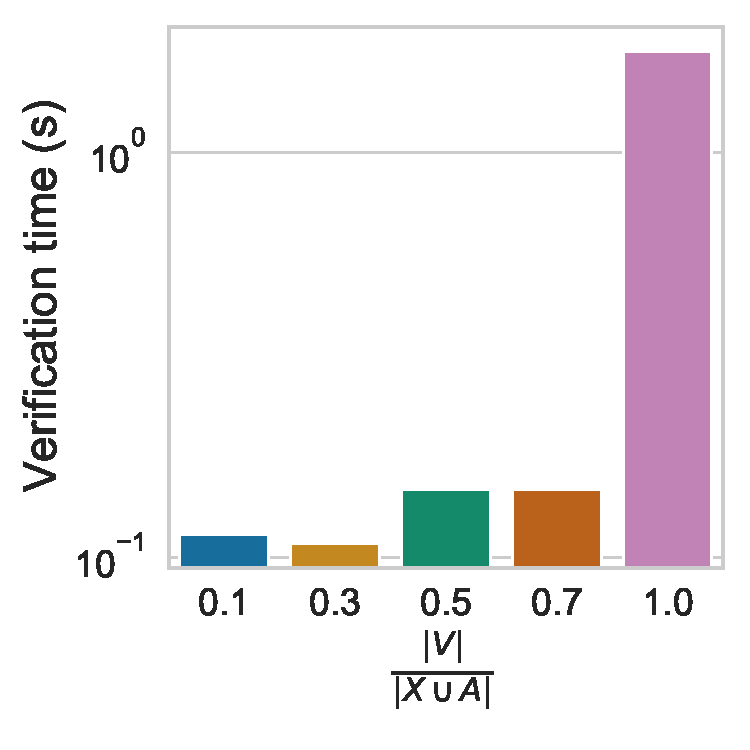
\includegraphics[scale=0.25]{figures/dag_complexity_DAG_time_Ricci_LR_Race__Position}}
%			\subfloat[]{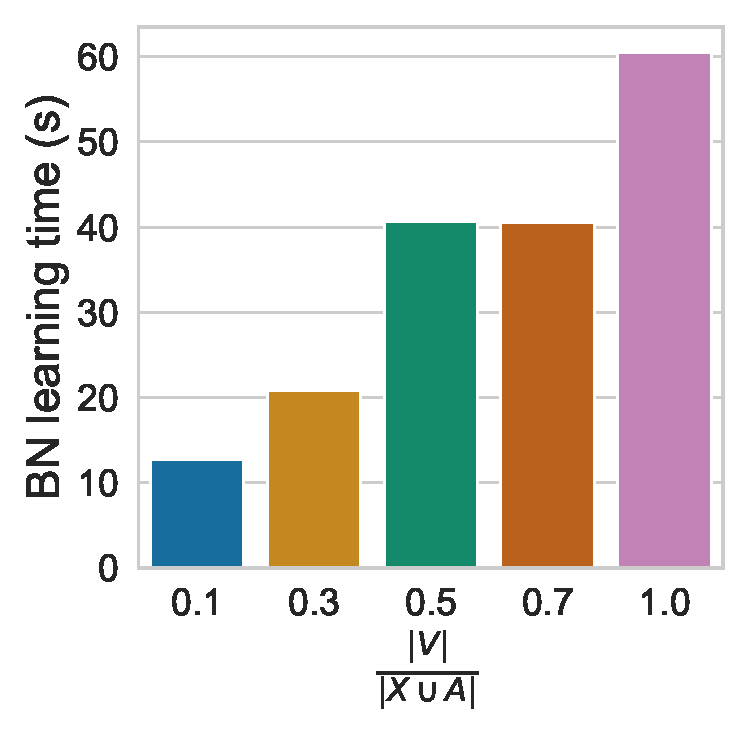
\includegraphics[scale=0.25]{figures/dag_complexity_DAG_time_notears_Ricci_LR_Race__Position}}
%			
	
	\subfloat{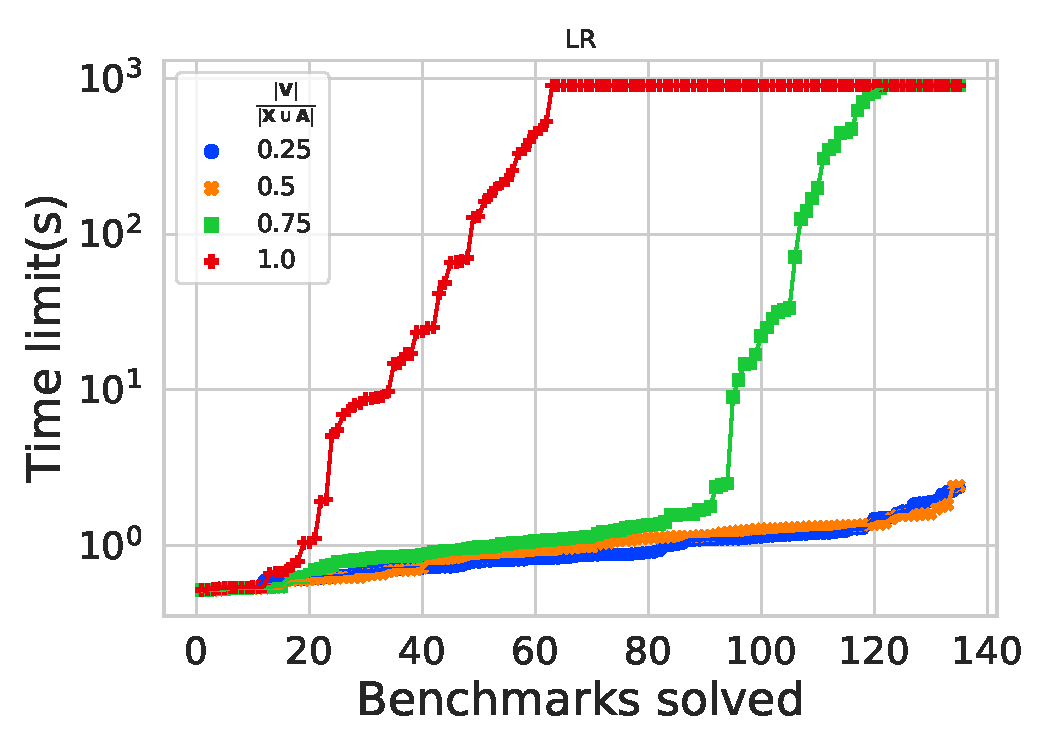
\includegraphics[scale=0.24]{figures/cactus_dag_LR_time}}
	\subfloat{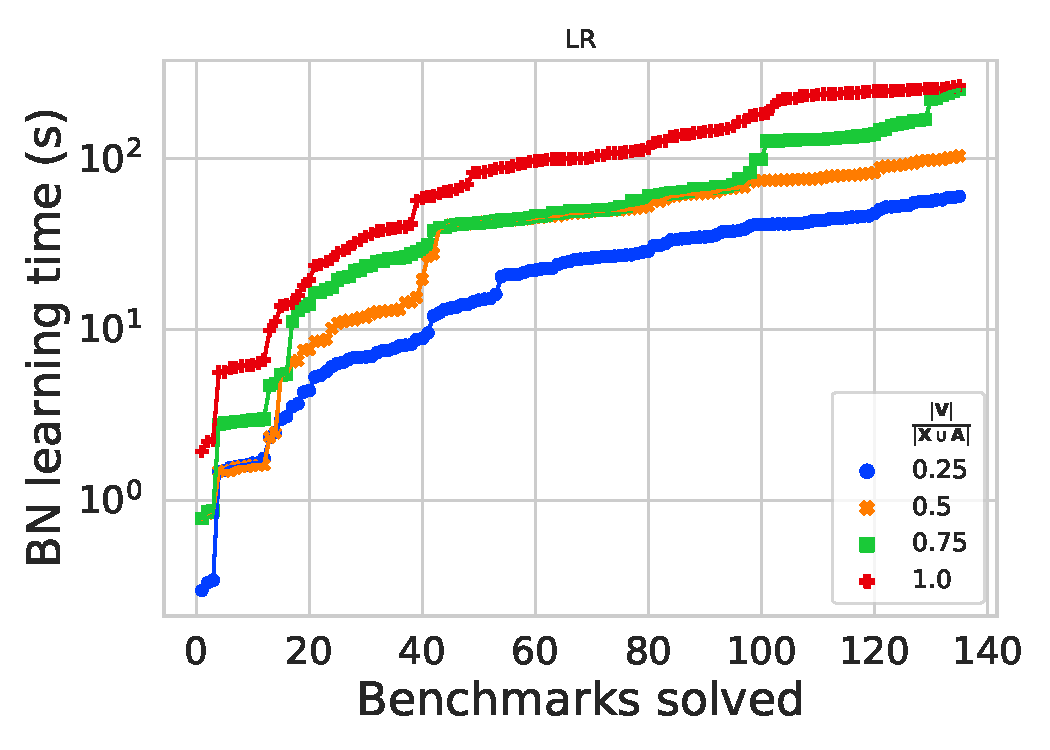
\includegraphics[scale=0.24]{figures/cactus_dag_LR_time_notears}}
			
		\end{center}
		
		\caption{Effect of number of variables in the learned Bayesian Network on computation time of {\framework}. In both plots, we vary $ \frac{|\mathbf{V}|}{|\nonsensitive \cup \sensitive|} $, that is the ratio between the number of variables in the Bayesian Network to the number of features. We observe that as this ratio increases to $ 1 $, both runtime of {\framework} (left plot) and network learning time (right plot) increase. } 
		\label{fig:results_DAG_complexity}
\end{figure}
	
	
	
